%
%===============>>  ГРУППА 9-1 МОДУЛЬ 9  <<=============
%
\setmodule{9}

%BEGIN_FOLD % ====>>_____ Занятие 1 _____<<====
\begin{class}[number=1]
	\begin{listofex}
		\item Найдите значение выражения: \(\dfrac{ 9,4 }{ 4,1+5,3 }\).
		\item На координатной прямой отмечены числа \( a \) и \( b \). Какое из следующих утверждений неверно?
		\begin{center}
			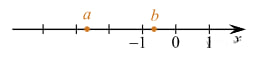
\includegraphics[align=t, width=0.5\linewidth]{\picpath/G93M8L6-6}
		\end{center}
		\begin{tasks}(2)
			\task \( a+b<0 \)
			\task \( -2<b-1<-1 \)
			\task \( a^2b<0 \)
			\task \( -a<0 \)
		\end{tasks}
		\item Найдите значение выражения \( \dfrac{a^{17}\cdot(b^5)^3}{(a\cdot b)^{15}} \) при \( a=7 \) и \( b=\sqrt{7} \).
		\item Решите уравнения: \(\dfrac{ 3 }{ x-19 }=\dfrac{ 19 }{ x-3 }\). \\
		Если корней несколько, запишите их в ответ без пробелов в порядке возрастания.
		\item В фирме такси в данный момент свободно \(15\) машин: \(3\) чёрных, \(6\) жёлтых и \(6\) зелёных. По вызову выехала одна из машин, случайно оказавшаяся ближе всего к заказчику. Найдите вероятность того, что к нему приедет жёлтое такси.
		\item На одном из рисунков изображен график функции \(y=x^2-2x+3\). Укажите номер этого рисунка.
		\begin{center}
			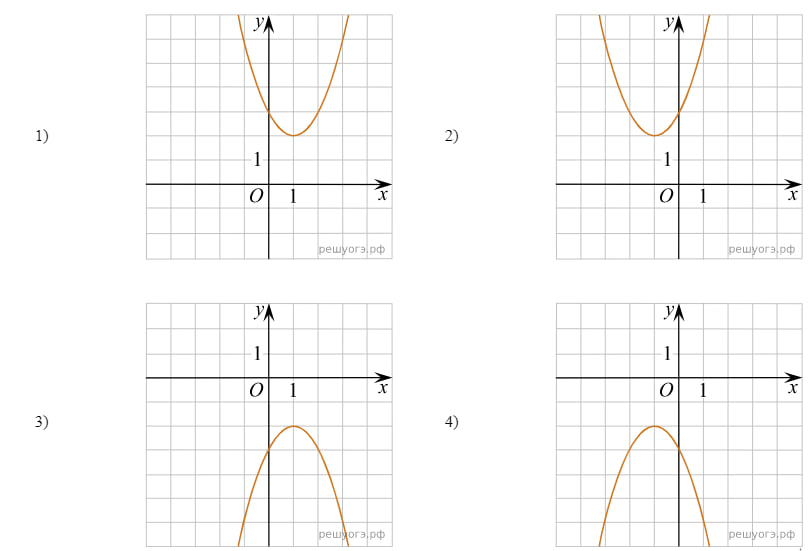
\includegraphics[align=t, width=0.5\linewidth]{\picpath/G91M9L1}
		\end{center}
		\item Объём пирамиды вычисляют по формуле \(V=\dfrac{ 1 }{ 3 }Sh\),  где \(S\) --- площадь основания пирамиды, \(h\) --- её высота. Объём пирамиды равен \(40\), площадь основания \(15\). Чему равна высота пирамиды?
		\item Решите неравенство: \(-x^2-2x\le0\).
		\item В амфитеатре \(14\) рядов. В первом ряду \(20\) мест, а в каждом следующем на \(3\) места больше, чем в предыдущем. Сколько мест в десятом ряду амфитеатра?
		\item В равностороннем треугольнике \(ABC\) биссектрисы \(CN\) и \(AM\) пересекаются в точке \(P\). Найдите \(\angle MPN\).
		\item К окружности с центром в точке \(O\) проведены касательная \(AB\) и секущая \(AO\). Найдите радиус окружности, если \(AB=12\) см, \(AO=13\) см.
		\item В треугольнике одна из сторон равна \(10\), другая равна \(10\sqrt{3}\), а угол между ними равен \(60\degree\). Найдите площадь треугольника.
		\item Основания трапеции равны \(18\) и \(12\), одна из боковых сторон равна \(4\sqrt{2}\), а угол между ней и одним из оснований равен \(135\degree\). Найдите площадь трапеции.
		\item Укажите номера верных утверждений.
		\begin{tasks}
			\task Если три угла одного треугольника равны трем углам другого треугольника, то такие треугольники подобны. 
			\task Сумма смежных углов равна \(180\degree\).
			\task Любая медиана равнобедренного треугольника является его биссектрисой.
		\end{tasks}
		\item Решите уравнение: \(x^2-2x+\sqrt{3-x}=\sqrt{3-x}+8\)
		\item Из пункта \(A\) в пункт \(B\), расстояние между которыми \(13\) км, вышел пешеход. Одновременно с ним из \(B\) в \(A\) выехал велосипедист. Велосипедист ехал со скоростью, на \(11\) км/ч большей скорости пешехода, и сделал в пути получасовую остановку. Найдите скорость пешехода, если известно, что они встретились в \(8\) км от пункта \(B\).
		\item Постройте график функции \(y=\dfrac{ (x+1)(x^2+7x+12) }{ x+3 }\) и определите, при каких значениях \(m\) прямая \(y=m\) имеет с графиком ровно одну общую точку.
		\item Периметр прямоугольника равен \(30\), а диагональ равна \(14\). Найдите площадь этого прямоугольника.
		\item Докажите, что медиана треугольника делит его на два треугольника, площади которых равны между собой.
	\end{listofex}
\end{class}
%END_FOLD

%BEGIN_FOLD % ====>>_____ Занятие 2 _____<<====
\begin{class}[number=2]
	\begin{listofex}
		\item Найдите значение выражения: \(0,6\cdot(-10)^3+50\).
		\item Какое из данных ниже чисел принадлежит промежутку \( [3;4] \)?
		\begin{tasks}(4)
			\task \( \dfrac{45}{19} \)
			\task \( \dfrac{52}{19} \)
			\task \( \dfrac{68}{19} \)
			\task \( \dfrac{77}{19} \)
		\end{tasks}
		\item Найдите значение выражения \( \dfrac{2c-4}{cd-2d} \) при \( c=0.5 \) и \(d=5 \).
		\item Решите уравнениe: \((x-4)^2+(x+9)^2\).
		\item Записан рост (в сантиметрах) пяти учащихся: \( 158 \), \( 166 \), \( 134 \), \( 130 \), \( 132 \). На сколько отличается среднее арифметическое этого набора чисел от его медианы?
		\item Найдите значение \( k \) по графику функции y=\(\dfrac{k}{x}\),  изображенному на рисунке.
		\begin{center}
			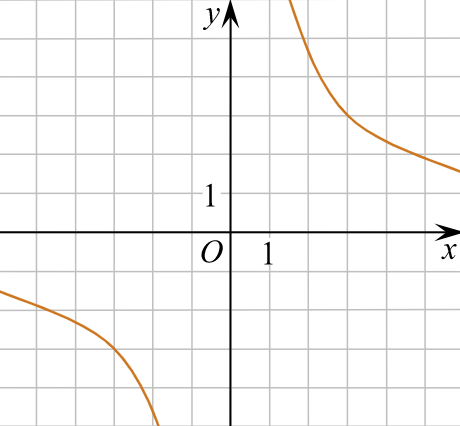
\includegraphics[align=t, width=0.3\linewidth]{\picpath/G91M9L2}
		\end{center}
		\item Радиус описанной около треугольника окружности можно найти по формуле \( R=\dfrac{a}{2\sin\alpha} \),  где \( a \) --- сторона треугольника, \( \alpha \) --- противолежащий этой стороне угол, а \( R \) --- радиус описанной около этого треугольника окружности. Пользуясь этой формулой, найдите \( \sin\alpha \), если \( a=0,6 \), а \( R=0,75 \).
		\item При каких значениях \( a \) выражение \( 5a+9 \) принимает отрицательные значения?
		\begin{tasks}(4)
			\task \( a>-\dfrac{9}{5} \)
			\task \( a<-\dfrac{5}{9} \)
			\task \( a>-\dfrac{5}{9} \)
			\task \( a><-\dfrac{9}{5} \)
		\end{tasks}
		\item У Кати есть попрыгунчик (каучуковый шарик). Она со всей силы бросила его об асфальт. После первого отскока попрыгунчик подлетел на высоту 400 см, а после каждого следующего отскока от асфальта подлетал на высоту в два раза меньше предыдущей. После какого по счёту отскока высота, на которую подлетит попрыгунчик, станет меньше \( 20 \) см?
		\item Площадь ромба равна \( 27 \), а периметр равен \( 36 \). Найдите высоту ромба.
		\item Прямоугольный треугольник с катетами \( 5 \) см и \( 12 \) см вписан в окружность. Чему равен радиус этой окружности?
		\item Основания равнобедренной трапеции равны \( 5 \) и \( 17 \), а ее боковые стороны равны \( 10 \). Найдите площадь трапеции.
		\item
		\begin{minipage}[t]{\bodywidth}
		На клетчатой бумаге с размером клетки \( 1X1 \) изображён треугольник \( ABC \). Найдите длину его средней линии, параллельной стороне \( AC \).
			\foranswer
		\end{minipage}
		\gapwidth
		\begin{minipage}[t]{\picwidth}
			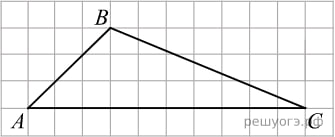
\includegraphics[align=t, width=\linewidth]{\picpath/G91M9L2-1}
		\end{minipage}
		\item Какие из следующих утверждений верны?
		\begin{tasks}
			\task Сумма углов выпуклого четырехугольника равна \( 180\degree \).
			\task Если один из углов параллелограмма равен 60°, то противоположный ему угол равен \( 120\degree \).
			\task Диагонали квадрата делят его углы пополам.
			\task Если в четырехугольнике две противоположные стороны равны, то этот четырехугольник --- параллелограмм.
		\end{tasks}
		\item Решите неравенство : \((\sqrt{3}-1,5)(3-2x)>0\)
		\item При смешивании первого раствора соли, концентрация которого \( 40\% \), и второго раствора этой же соли, концентрация которого \( 48\% \), получился раствор с концентрацией \( 42\% \). В каком отношении были взяты первый и второй растворы?
		\item Постройте график функции \(y=\dfrac{x-2}{(\sqrt{x^2-2x})^2}\) и найдите все значения \( k \), при которых прямая \( y=kx \) имеет с графиком данной функции ровно одну общую точку.
		\item Прямая, параллельная основаниям \( MP \) и \( NK \) трапеции \( MNKP \), проходит через точку пересечения диагоналей трапеции и пересекает её боковые стороны \( MN \) и \( KP \) в точках  \( A \) и \( B \) соответственно. Найдите длину отрезка \( AB \), если \( MP=40 \) см, \( NK=24 \) см.
		\item Дан правильный восьмиугольник. Докажите, что если его вершины последовательно соединить отрезками через одну, то получится квадрат.
	\end{listofex}
\end{class}
%END_FOLD

%BEGIN_FOLD % ====>>_ Домашняя работа 1 _<<====
\begin{homework}[number=1]
	\begin{listofex}
		\item Найдите значение выражения: \(\dfrac{9,4}{4,1+5,3}\).
		\item О числах \( a \), \( b\), \( c \) и \( d \) известно, что \( a<b \), \( b=c \), \( d>c \). Сравнитe числа \( d \) и \( a \).
		\begin{tasks}(4)
			\task \( d=a \)
			\task \( d>a \)
			\task \( d<a \)
			\task Сравнить невозможно.
		\end{tasks}
		\item Найдите значение выражения \( \sqrt{7\cdot12}\cdot\sqrt{21} \).
		\item Решите уравнениe: \(\dfrac{x}{4}+x=4\).
		\item Миша с папой решили покататься на колесе обозрения. Всего на колесе пятнадцать кабинок, из них \( 2 \) --- синие, \( 10 \) --- зеленые, остальные  --- красные. Кабинки по очереди подходят к платформе для посадки. Найдите вероятность того, что Миша прокатится в красной кабинке.
		\item Установите соответствие между графиками функций и формулами, которые их задают.
		\begin{center}
			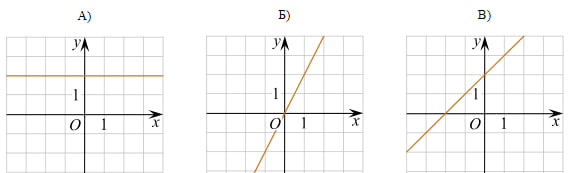
\includegraphics[align=t, width=0.8\linewidth]{\picpath/G91M9H1}
		\end{center}
		\begin{tasks}(4)
			\task \( y=2x \)
			\task \( y=-2x \)
			\task \( y=x+2 \)
			\task \( y=2 \)
		\end{tasks}
		\item Полную механическую энергию тела (в джоулях) можно вычислить по формуле \( E=\dfrac{mv^2}{2}+mgh \),  где \( m \) --- масса тела (в килограммах), \( v \) --- его скорость (в м/с), \( h \) --- высота положения центра масс тела над произвольно выбранным нулевым уровнем (в метрах), а \( g \) --- ускорение свободного падения (в м/с\( ^2 \)). Пользуясь этой формулой, найдите \( m \) (в килограммах), если \( E=336 \) Дж,  \( v=6 \) м/с, \( h=3 \) м, а \( g=10 \) м/с\( ^2 \). 
		\item Решите неравенство: \( \dfrac{x-2}{3-x}\ge0 \)
		\item Бригада маляров красит забор длиной \( 240 \) метров, ежедневно увеличивая норму покраски на одно и то же число метров. Известно, что за первый и последний день в сумме бригада покрасила \( 60 \) метров забора. Определите, сколько дней бригада маляров красила весь забор.
		\item В равнобедренном треугольнике \( ABC \) \( AC=BC \). Найдите \( AC \), если высота \( CH=12 \), \( AB=10 \).
		\item На отрезке \( AB \) выбрана точка \( C \) так, что \( AC=75 \) и \( BC=10 \). Построена окружность с центром \( A \), проходящая через \( C \). Найдите длину отрезка касательной, проведённой из точки \( B \) к этой окружности.
		\item
		\begin{minipage}[t]{\bodywidth}
			Площадь одной клетки равна \( 1 \). Найдите площадь фигуры, изображённой на рисунке.
			\foranswer
		\end{minipage}
		\gapwidth
		\begin{minipage}[t]{\picwidth}
			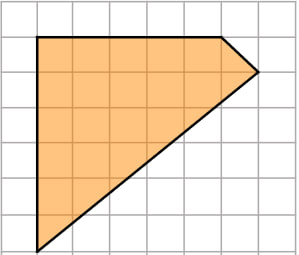
\includegraphics[align=t, width=\linewidth]{\picpath/G91M9H1-1}
		\end{minipage}
		\item Какие из следующих утверждений верны?
		\begin{tasks}
			\task Окружность имеет бесконечно много центров симметрии.
			\task Прямая не имеет осей симметрии.
			\task Правильный пятиугольник имеет пять осей симметрии.
			\task Квадрат не имеет центра симметрии.
		\end{tasks}
	\end{listofex}
\end{homework}
%END_FOLD

%BEGIN_FOLD % ====>>_____ Занятие 3 _____<<====
\begin{class}[number=3]
	\begin{listofex}
		\item Найдите значение выражения: \(3\cdot10^{-1}+1\cdot10^{-2}+5\cdot10^{-4}\).
		\item Какое из приведенных ниже неравенств является верным при любых значениях \( a \) и \( b \), удовлетворяющих условию \( a>b \)?
		\begin{tasks}(4)
			\task \( b-a<-2 \)
			\task \( a-b>-1 \)
			\task \( a-b<3 \)
			\task \( b-a>-3 \)
		\end{tasks}
		\item Упростите выражение \( \dfrac{x^2-4}{4x^2}\cdot\dfrac{2x}{x+2} \) и найдите его значение при \( x=4 \). В ответ запишите полученное число.
		\item Решите уравнениe: \(\dfrac{6}{x-8}=\dfrac{8}{x-6}\).
		\item Телевизор у Любы сломался и показывает только один случайный канал. Люба включает телевизор. В это время по двадцати пяти каналам из пятидесяти показывают кинокомедии. Найдите вероятность того, что Люба попадет на канал, где комедия не идет.
		\item График какой из приведенных ниже функций изображен на рисунке?
		\begin{center}
			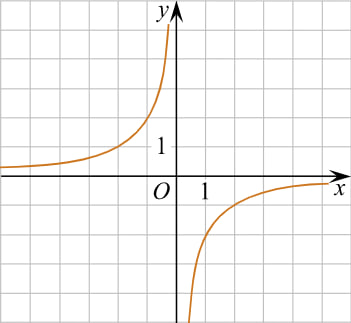
\includegraphics[align=t, width=0.3\linewidth]{\picpath/G91M9L3}
		\end{center}
		\begin{tasks}(4)
			\task \( y=-\dfrac{2}{x} \)
			\task \( y=\dfrac{2}{x} \)
			\task \( y=-\dfrac{1}{2x} \)
			\task \( y=\dfrac{1}{2x} \)
		\end{tasks}
		\item Чтобы перевести значение температуры по шкале Цельсия (\( t\degree C \)) в шкалу Фаренгейта (\( t\degree F \)), пользуются формулой \( F=1,8C+32 \), где \( C \) --- градусы Цельсия, \( F \) --- градусы Фаренгейта. Какая температура по шкале Фаренгейта соответствует \( 111\degree \) по шкале Цельсия?
		\item Решите неравенство: \( x^2-4x+3\ge0 \).
		\item В амфитеатре \( 23 \) ряда, причём в каждом следующем ряду на одно и то же число мест больше, чем в предыдущем. В седьмом ряду \( 26 \) мест,	а в одиннадцатом ряду \( 34 \) места. Сколько мест в последнем ряду амфитеатра?
		\item Один угол параллелограмма в одиннадцать раз больше другого. Найдите меньший угол. Ответ дайте в градусах.
		\item В окружности с центром в точке \( O \) проведены диаметры \( AD \) и \( BC \), угол \( OCD \) равен \( 30\degree \). Найдите величину угла \( OAB \).
		\item 
		\begin{minipage}[t]{\bodywidth}
			Найдите площадь трапеции, изображённой на рисунке.
			\foranswer
		\end{minipage}
		\gapwidth
		\begin{minipage}[t]{\picwidth}
			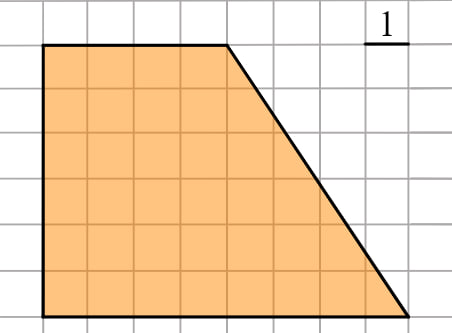
\includegraphics[align=t, width=\linewidth]{\picpath/G91M9L3-1}
		\end{minipage}
		\item
		\begin{minipage}[t]{\bodywidth}
			Найдите угол \( ABC \). Ответ дайте в градусах.
			\foranswer
		\end{minipage}
		\gapwidth
		\begin{minipage}[t]{\picwidth}
			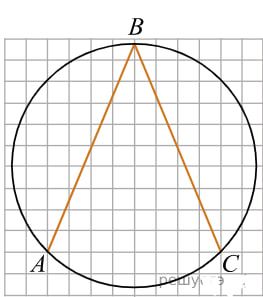
\includegraphics[align=t, width=\linewidth]{\picpath/G91M9L3-2}
		\end{minipage}
		\item Какие из следующих утверждений верны?
		\begin{tasks}
			\task Если при пересечении двух прямых третьей прямой внутренние накрест лежащие углы составляют в сумме \( 90\degree \), то эти две прямые параллельны.
			\task Если угол равен \( 60\degree \), то смежный с ним равен \( 120\degree \).
			\task Если при пересечении двух прямых третьей прямой внутренние односторонние углы равны \( 70\degree \) и \( 110\degree \), то эти две прямые параллельны.
			\task Через любые три точки проходит не более одной прямой.
		\end{tasks}
		\item Решите уравнение: \((x^2-9)^2+(x^2-2x-15)^2=0\)
		\item Из пунктов \( A \) и \( B \), расстояние между которыми \( 19 \) км, вышли одновременно навстречу друг другу два пешехода и встретились в \( 9 \) км от \( A \). Найдите скорость пешехода, шедшего из \( A \), если известно, что он шёл со скоростью, на \( 1 \) км/ч большей, чем пешеход, шедший из \( B \), и сделал в пути получасовую остановку.
		\item Постройте график функции \(y=\dfrac{(x+1)(x^2+7x+12)}{x+3}\) и найдите все значения \( m \), при которых прямая \( y=m \) имеет с графиком данной функции ровно одну общую точку.
		\item В трапеции \( ABCD \) основание \( AD \) вдвое больше основания \( BC \) и вдвое больше боковой стороны \( CD \). Угол \( ADC \) равен \( 60\degree \), сторона \( AB \) равна \( 4 \). Найдите площадь трапеции.
		\item В треугольнике \( ABC \) угол \( B \) равен \( 36\degree \), \( AB=BC \), \( AD \) --- биссектриса. Докажите, что треугольник \( ABD \) --- равнобедренный.
	\end{listofex}
\end{class}
%END_FOLD

%BEGIN_FOLD % ====>>_____ Занятие 4 _____<<====
\begin{class}[number=4]
	\begin{listofex}
		\item Занятие 4
	\end{listofex}
\end{class}
%END_FOLD

%BEGIN_FOLD % ====>>_ Домашняя работа 2 _<<====
\begin{homework}[number=2]
	\begin{listofex}
		\item .
	\end{listofex}
\end{homework}
%END_FOLD

%BEGIN_FOLD % ====>>_____ Занятие 5 _____<<====
\begin{class}[number=5]
	\begin{listofex}
		\item .
	\end{listofex}
\end{class}
%END_FOLD

%BEGIN_FOLD % ====>>_____ Занятие 6 _____<<====
\begin{class}[number=6]
	\begin{listofex}
		\item .
	\end{listofex}
\end{class}
%END_FOLD

%BEGIN_FOLD % ====>>_ Домашняя работа 3 _<<====
\begin{homework}[number=3]
	\begin{listofex}
		\item .
	\end{listofex}
\end{homework}
%END_FOLD

%BEGIN_FOLD % ====>>_____ Занятие 7 _____<<====
\begin{class}[number=7]
	\begin{listofex}
		\item .
	\end{listofex}
\end{class}
%END_FOLD

%BEGIN_FOLD % ====>>_ Проверочная работа _<<====
\begin{class}[number=8]
	\begin{listofex}
		\item .
	\end{listofex}
\end{class}
%END_FOLD